\documentclass[letter]{article}\usepackage{graphicx, color}
%% maxwidth is the original width if it is less than linewidth
%% otherwise use linewidth (to make sure the graphics do not exceed the margin)
\makeatletter
\def\maxwidth{ %
  \ifdim\Gin@nat@width>\linewidth
    \linewidth
  \else
    \Gin@nat@width
  \fi
}
\makeatother

\IfFileExists{upquote.sty}{\usepackage{upquote}}{}
\definecolor{fgcolor}{rgb}{0.267, 0.267, 0.267}
\newcommand{\hlnumber}[1]{\textcolor[rgb]{0,0,0}{#1}}%
\newcommand{\hlfunctioncall}[1]{\textcolor[rgb]{0.501960784313725,0,0.329411764705882}{\textbf{#1}}}%
\newcommand{\hlstring}[1]{\textcolor[rgb]{0.6,0.6,1}{#1}}%
\newcommand{\hlkeyword}[1]{\textcolor[rgb]{0,0,0}{\textbf{#1}}}%
\newcommand{\hlargument}[1]{\textcolor[rgb]{0.690196078431373,0.250980392156863,0.0196078431372549}{#1}}%
\newcommand{\hlcomment}[1]{\textcolor[rgb]{0.180392156862745,0.6,0.341176470588235}{#1}}%
\newcommand{\hlroxygencomment}[1]{\textcolor[rgb]{0.43921568627451,0.47843137254902,0.701960784313725}{#1}}%
\newcommand{\hlformalargs}[1]{\textcolor[rgb]{0.690196078431373,0.250980392156863,0.0196078431372549}{#1}}%
\newcommand{\hleqformalargs}[1]{\textcolor[rgb]{0.690196078431373,0.250980392156863,0.0196078431372549}{#1}}%
\newcommand{\hlassignement}[1]{\textcolor[rgb]{0,0,0}{\textbf{#1}}}%
\newcommand{\hlpackage}[1]{\textcolor[rgb]{0.588235294117647,0.709803921568627,0.145098039215686}{#1}}%
\newcommand{\hlslot}[1]{\textit{#1}}%
\newcommand{\hlsymbol}[1]{\textcolor[rgb]{0,0,0}{#1}}%
\newcommand{\hlprompt}[1]{\textcolor[rgb]{0.266666666666667,0.266666666666667,0.266666666666667}{#1}}%

\usepackage{color}%
 
\newsavebox{\hlnormalsizeboxclosebrace}%
\newsavebox{\hlnormalsizeboxopenbrace}%
\newsavebox{\hlnormalsizeboxbackslash}%
\newsavebox{\hlnormalsizeboxlessthan}%
\newsavebox{\hlnormalsizeboxgreaterthan}%
\newsavebox{\hlnormalsizeboxdollar}%
\newsavebox{\hlnormalsizeboxunderscore}%
\newsavebox{\hlnormalsizeboxand}%
\newsavebox{\hlnormalsizeboxhash}%
\newsavebox{\hlnormalsizeboxat}%
\newsavebox{\hlnormalsizeboxpercent}% 
\newsavebox{\hlnormalsizeboxhat}%
\newsavebox{\hlnormalsizeboxsinglequote}%
\newsavebox{\hlnormalsizeboxbacktick}%

\setbox\hlnormalsizeboxopenbrace=\hbox{\begin{normalsize}\verb.{.\end{normalsize}}%
\setbox\hlnormalsizeboxclosebrace=\hbox{\begin{normalsize}\verb.}.\end{normalsize}}%
\setbox\hlnormalsizeboxlessthan=\hbox{\begin{normalsize}\verb.<.\end{normalsize}}%
\setbox\hlnormalsizeboxdollar=\hbox{\begin{normalsize}\verb.$.\end{normalsize}}%
\setbox\hlnormalsizeboxunderscore=\hbox{\begin{normalsize}\verb._.\end{normalsize}}%
\setbox\hlnormalsizeboxand=\hbox{\begin{normalsize}\verb.&.\end{normalsize}}%
\setbox\hlnormalsizeboxhash=\hbox{\begin{normalsize}\verb.#.\end{normalsize}}%
\setbox\hlnormalsizeboxat=\hbox{\begin{normalsize}\verb.@.\end{normalsize}}%
\setbox\hlnormalsizeboxbackslash=\hbox{\begin{normalsize}\verb.\.\end{normalsize}}%
\setbox\hlnormalsizeboxgreaterthan=\hbox{\begin{normalsize}\verb.>.\end{normalsize}}%
\setbox\hlnormalsizeboxpercent=\hbox{\begin{normalsize}\verb.%.\end{normalsize}}%
\setbox\hlnormalsizeboxhat=\hbox{\begin{normalsize}\verb.^.\end{normalsize}}%
\setbox\hlnormalsizeboxsinglequote=\hbox{\begin{normalsize}\verb.'.\end{normalsize}}%
\setbox\hlnormalsizeboxbacktick=\hbox{\begin{normalsize}\verb.`.\end{normalsize}}%
\setbox\hlnormalsizeboxhat=\hbox{\begin{normalsize}\verb.^.\end{normalsize}}%



\newsavebox{\hltinyboxclosebrace}%
\newsavebox{\hltinyboxopenbrace}%
\newsavebox{\hltinyboxbackslash}%
\newsavebox{\hltinyboxlessthan}%
\newsavebox{\hltinyboxgreaterthan}%
\newsavebox{\hltinyboxdollar}%
\newsavebox{\hltinyboxunderscore}%
\newsavebox{\hltinyboxand}%
\newsavebox{\hltinyboxhash}%
\newsavebox{\hltinyboxat}%
\newsavebox{\hltinyboxpercent}% 
\newsavebox{\hltinyboxhat}%
\newsavebox{\hltinyboxsinglequote}%
\newsavebox{\hltinyboxbacktick}%

\setbox\hltinyboxopenbrace=\hbox{\begin{tiny}\verb.{.\end{tiny}}%
\setbox\hltinyboxclosebrace=\hbox{\begin{tiny}\verb.}.\end{tiny}}%
\setbox\hltinyboxlessthan=\hbox{\begin{tiny}\verb.<.\end{tiny}}%
\setbox\hltinyboxdollar=\hbox{\begin{tiny}\verb.$.\end{tiny}}%
\setbox\hltinyboxunderscore=\hbox{\begin{tiny}\verb._.\end{tiny}}%
\setbox\hltinyboxand=\hbox{\begin{tiny}\verb.&.\end{tiny}}%
\setbox\hltinyboxhash=\hbox{\begin{tiny}\verb.#.\end{tiny}}%
\setbox\hltinyboxat=\hbox{\begin{tiny}\verb.@.\end{tiny}}%
\setbox\hltinyboxbackslash=\hbox{\begin{tiny}\verb.\.\end{tiny}}%
\setbox\hltinyboxgreaterthan=\hbox{\begin{tiny}\verb.>.\end{tiny}}%
\setbox\hltinyboxpercent=\hbox{\begin{tiny}\verb.%.\end{tiny}}%
\setbox\hltinyboxhat=\hbox{\begin{tiny}\verb.^.\end{tiny}}%
\setbox\hltinyboxsinglequote=\hbox{\begin{tiny}\verb.'.\end{tiny}}%
\setbox\hltinyboxbacktick=\hbox{\begin{tiny}\verb.`.\end{tiny}}%
\setbox\hltinyboxhat=\hbox{\begin{tiny}\verb.^.\end{tiny}}%



\newsavebox{\hlscriptsizeboxclosebrace}%
\newsavebox{\hlscriptsizeboxopenbrace}%
\newsavebox{\hlscriptsizeboxbackslash}%
\newsavebox{\hlscriptsizeboxlessthan}%
\newsavebox{\hlscriptsizeboxgreaterthan}%
\newsavebox{\hlscriptsizeboxdollar}%
\newsavebox{\hlscriptsizeboxunderscore}%
\newsavebox{\hlscriptsizeboxand}%
\newsavebox{\hlscriptsizeboxhash}%
\newsavebox{\hlscriptsizeboxat}%
\newsavebox{\hlscriptsizeboxpercent}% 
\newsavebox{\hlscriptsizeboxhat}%
\newsavebox{\hlscriptsizeboxsinglequote}%
\newsavebox{\hlscriptsizeboxbacktick}%

\setbox\hlscriptsizeboxopenbrace=\hbox{\begin{scriptsize}\verb.{.\end{scriptsize}}%
\setbox\hlscriptsizeboxclosebrace=\hbox{\begin{scriptsize}\verb.}.\end{scriptsize}}%
\setbox\hlscriptsizeboxlessthan=\hbox{\begin{scriptsize}\verb.<.\end{scriptsize}}%
\setbox\hlscriptsizeboxdollar=\hbox{\begin{scriptsize}\verb.$.\end{scriptsize}}%
\setbox\hlscriptsizeboxunderscore=\hbox{\begin{scriptsize}\verb._.\end{scriptsize}}%
\setbox\hlscriptsizeboxand=\hbox{\begin{scriptsize}\verb.&.\end{scriptsize}}%
\setbox\hlscriptsizeboxhash=\hbox{\begin{scriptsize}\verb.#.\end{scriptsize}}%
\setbox\hlscriptsizeboxat=\hbox{\begin{scriptsize}\verb.@.\end{scriptsize}}%
\setbox\hlscriptsizeboxbackslash=\hbox{\begin{scriptsize}\verb.\.\end{scriptsize}}%
\setbox\hlscriptsizeboxgreaterthan=\hbox{\begin{scriptsize}\verb.>.\end{scriptsize}}%
\setbox\hlscriptsizeboxpercent=\hbox{\begin{scriptsize}\verb.%.\end{scriptsize}}%
\setbox\hlscriptsizeboxhat=\hbox{\begin{scriptsize}\verb.^.\end{scriptsize}}%
\setbox\hlscriptsizeboxsinglequote=\hbox{\begin{scriptsize}\verb.'.\end{scriptsize}}%
\setbox\hlscriptsizeboxbacktick=\hbox{\begin{scriptsize}\verb.`.\end{scriptsize}}%
\setbox\hlscriptsizeboxhat=\hbox{\begin{scriptsize}\verb.^.\end{scriptsize}}%



\newsavebox{\hlfootnotesizeboxclosebrace}%
\newsavebox{\hlfootnotesizeboxopenbrace}%
\newsavebox{\hlfootnotesizeboxbackslash}%
\newsavebox{\hlfootnotesizeboxlessthan}%
\newsavebox{\hlfootnotesizeboxgreaterthan}%
\newsavebox{\hlfootnotesizeboxdollar}%
\newsavebox{\hlfootnotesizeboxunderscore}%
\newsavebox{\hlfootnotesizeboxand}%
\newsavebox{\hlfootnotesizeboxhash}%
\newsavebox{\hlfootnotesizeboxat}%
\newsavebox{\hlfootnotesizeboxpercent}% 
\newsavebox{\hlfootnotesizeboxhat}%
\newsavebox{\hlfootnotesizeboxsinglequote}%
\newsavebox{\hlfootnotesizeboxbacktick}%

\setbox\hlfootnotesizeboxopenbrace=\hbox{\begin{footnotesize}\verb.{.\end{footnotesize}}%
\setbox\hlfootnotesizeboxclosebrace=\hbox{\begin{footnotesize}\verb.}.\end{footnotesize}}%
\setbox\hlfootnotesizeboxlessthan=\hbox{\begin{footnotesize}\verb.<.\end{footnotesize}}%
\setbox\hlfootnotesizeboxdollar=\hbox{\begin{footnotesize}\verb.$.\end{footnotesize}}%
\setbox\hlfootnotesizeboxunderscore=\hbox{\begin{footnotesize}\verb._.\end{footnotesize}}%
\setbox\hlfootnotesizeboxand=\hbox{\begin{footnotesize}\verb.&.\end{footnotesize}}%
\setbox\hlfootnotesizeboxhash=\hbox{\begin{footnotesize}\verb.#.\end{footnotesize}}%
\setbox\hlfootnotesizeboxat=\hbox{\begin{footnotesize}\verb.@.\end{footnotesize}}%
\setbox\hlfootnotesizeboxbackslash=\hbox{\begin{footnotesize}\verb.\.\end{footnotesize}}%
\setbox\hlfootnotesizeboxgreaterthan=\hbox{\begin{footnotesize}\verb.>.\end{footnotesize}}%
\setbox\hlfootnotesizeboxpercent=\hbox{\begin{footnotesize}\verb.%.\end{footnotesize}}%
\setbox\hlfootnotesizeboxhat=\hbox{\begin{footnotesize}\verb.^.\end{footnotesize}}%
\setbox\hlfootnotesizeboxsinglequote=\hbox{\begin{footnotesize}\verb.'.\end{footnotesize}}%
\setbox\hlfootnotesizeboxbacktick=\hbox{\begin{footnotesize}\verb.`.\end{footnotesize}}%
\setbox\hlfootnotesizeboxhat=\hbox{\begin{footnotesize}\verb.^.\end{footnotesize}}%



\newsavebox{\hlsmallboxclosebrace}%
\newsavebox{\hlsmallboxopenbrace}%
\newsavebox{\hlsmallboxbackslash}%
\newsavebox{\hlsmallboxlessthan}%
\newsavebox{\hlsmallboxgreaterthan}%
\newsavebox{\hlsmallboxdollar}%
\newsavebox{\hlsmallboxunderscore}%
\newsavebox{\hlsmallboxand}%
\newsavebox{\hlsmallboxhash}%
\newsavebox{\hlsmallboxat}%
\newsavebox{\hlsmallboxpercent}% 
\newsavebox{\hlsmallboxhat}%
\newsavebox{\hlsmallboxsinglequote}%
\newsavebox{\hlsmallboxbacktick}%

\setbox\hlsmallboxopenbrace=\hbox{\begin{small}\verb.{.\end{small}}%
\setbox\hlsmallboxclosebrace=\hbox{\begin{small}\verb.}.\end{small}}%
\setbox\hlsmallboxlessthan=\hbox{\begin{small}\verb.<.\end{small}}%
\setbox\hlsmallboxdollar=\hbox{\begin{small}\verb.$.\end{small}}%
\setbox\hlsmallboxunderscore=\hbox{\begin{small}\verb._.\end{small}}%
\setbox\hlsmallboxand=\hbox{\begin{small}\verb.&.\end{small}}%
\setbox\hlsmallboxhash=\hbox{\begin{small}\verb.#.\end{small}}%
\setbox\hlsmallboxat=\hbox{\begin{small}\verb.@.\end{small}}%
\setbox\hlsmallboxbackslash=\hbox{\begin{small}\verb.\.\end{small}}%
\setbox\hlsmallboxgreaterthan=\hbox{\begin{small}\verb.>.\end{small}}%
\setbox\hlsmallboxpercent=\hbox{\begin{small}\verb.%.\end{small}}%
\setbox\hlsmallboxhat=\hbox{\begin{small}\verb.^.\end{small}}%
\setbox\hlsmallboxsinglequote=\hbox{\begin{small}\verb.'.\end{small}}%
\setbox\hlsmallboxbacktick=\hbox{\begin{small}\verb.`.\end{small}}%
\setbox\hlsmallboxhat=\hbox{\begin{small}\verb.^.\end{small}}%



\newsavebox{\hllargeboxclosebrace}%
\newsavebox{\hllargeboxopenbrace}%
\newsavebox{\hllargeboxbackslash}%
\newsavebox{\hllargeboxlessthan}%
\newsavebox{\hllargeboxgreaterthan}%
\newsavebox{\hllargeboxdollar}%
\newsavebox{\hllargeboxunderscore}%
\newsavebox{\hllargeboxand}%
\newsavebox{\hllargeboxhash}%
\newsavebox{\hllargeboxat}%
\newsavebox{\hllargeboxpercent}% 
\newsavebox{\hllargeboxhat}%
\newsavebox{\hllargeboxsinglequote}%
\newsavebox{\hllargeboxbacktick}%

\setbox\hllargeboxopenbrace=\hbox{\begin{large}\verb.{.\end{large}}%
\setbox\hllargeboxclosebrace=\hbox{\begin{large}\verb.}.\end{large}}%
\setbox\hllargeboxlessthan=\hbox{\begin{large}\verb.<.\end{large}}%
\setbox\hllargeboxdollar=\hbox{\begin{large}\verb.$.\end{large}}%
\setbox\hllargeboxunderscore=\hbox{\begin{large}\verb._.\end{large}}%
\setbox\hllargeboxand=\hbox{\begin{large}\verb.&.\end{large}}%
\setbox\hllargeboxhash=\hbox{\begin{large}\verb.#.\end{large}}%
\setbox\hllargeboxat=\hbox{\begin{large}\verb.@.\end{large}}%
\setbox\hllargeboxbackslash=\hbox{\begin{large}\verb.\.\end{large}}%
\setbox\hllargeboxgreaterthan=\hbox{\begin{large}\verb.>.\end{large}}%
\setbox\hllargeboxpercent=\hbox{\begin{large}\verb.%.\end{large}}%
\setbox\hllargeboxhat=\hbox{\begin{large}\verb.^.\end{large}}%
\setbox\hllargeboxsinglequote=\hbox{\begin{large}\verb.'.\end{large}}%
\setbox\hllargeboxbacktick=\hbox{\begin{large}\verb.`.\end{large}}%
\setbox\hllargeboxhat=\hbox{\begin{large}\verb.^.\end{large}}%



\newsavebox{\hlLargeboxclosebrace}%
\newsavebox{\hlLargeboxopenbrace}%
\newsavebox{\hlLargeboxbackslash}%
\newsavebox{\hlLargeboxlessthan}%
\newsavebox{\hlLargeboxgreaterthan}%
\newsavebox{\hlLargeboxdollar}%
\newsavebox{\hlLargeboxunderscore}%
\newsavebox{\hlLargeboxand}%
\newsavebox{\hlLargeboxhash}%
\newsavebox{\hlLargeboxat}%
\newsavebox{\hlLargeboxpercent}% 
\newsavebox{\hlLargeboxhat}%
\newsavebox{\hlLargeboxsinglequote}%
\newsavebox{\hlLargeboxbacktick}%

\setbox\hlLargeboxopenbrace=\hbox{\begin{Large}\verb.{.\end{Large}}%
\setbox\hlLargeboxclosebrace=\hbox{\begin{Large}\verb.}.\end{Large}}%
\setbox\hlLargeboxlessthan=\hbox{\begin{Large}\verb.<.\end{Large}}%
\setbox\hlLargeboxdollar=\hbox{\begin{Large}\verb.$.\end{Large}}%
\setbox\hlLargeboxunderscore=\hbox{\begin{Large}\verb._.\end{Large}}%
\setbox\hlLargeboxand=\hbox{\begin{Large}\verb.&.\end{Large}}%
\setbox\hlLargeboxhash=\hbox{\begin{Large}\verb.#.\end{Large}}%
\setbox\hlLargeboxat=\hbox{\begin{Large}\verb.@.\end{Large}}%
\setbox\hlLargeboxbackslash=\hbox{\begin{Large}\verb.\.\end{Large}}%
\setbox\hlLargeboxgreaterthan=\hbox{\begin{Large}\verb.>.\end{Large}}%
\setbox\hlLargeboxpercent=\hbox{\begin{Large}\verb.%.\end{Large}}%
\setbox\hlLargeboxhat=\hbox{\begin{Large}\verb.^.\end{Large}}%
\setbox\hlLargeboxsinglequote=\hbox{\begin{Large}\verb.'.\end{Large}}%
\setbox\hlLargeboxbacktick=\hbox{\begin{Large}\verb.`.\end{Large}}%
\setbox\hlLargeboxhat=\hbox{\begin{Large}\verb.^.\end{Large}}%



\newsavebox{\hlLARGEboxclosebrace}%
\newsavebox{\hlLARGEboxopenbrace}%
\newsavebox{\hlLARGEboxbackslash}%
\newsavebox{\hlLARGEboxlessthan}%
\newsavebox{\hlLARGEboxgreaterthan}%
\newsavebox{\hlLARGEboxdollar}%
\newsavebox{\hlLARGEboxunderscore}%
\newsavebox{\hlLARGEboxand}%
\newsavebox{\hlLARGEboxhash}%
\newsavebox{\hlLARGEboxat}%
\newsavebox{\hlLARGEboxpercent}% 
\newsavebox{\hlLARGEboxhat}%
\newsavebox{\hlLARGEboxsinglequote}%
\newsavebox{\hlLARGEboxbacktick}%

\setbox\hlLARGEboxopenbrace=\hbox{\begin{LARGE}\verb.{.\end{LARGE}}%
\setbox\hlLARGEboxclosebrace=\hbox{\begin{LARGE}\verb.}.\end{LARGE}}%
\setbox\hlLARGEboxlessthan=\hbox{\begin{LARGE}\verb.<.\end{LARGE}}%
\setbox\hlLARGEboxdollar=\hbox{\begin{LARGE}\verb.$.\end{LARGE}}%
\setbox\hlLARGEboxunderscore=\hbox{\begin{LARGE}\verb._.\end{LARGE}}%
\setbox\hlLARGEboxand=\hbox{\begin{LARGE}\verb.&.\end{LARGE}}%
\setbox\hlLARGEboxhash=\hbox{\begin{LARGE}\verb.#.\end{LARGE}}%
\setbox\hlLARGEboxat=\hbox{\begin{LARGE}\verb.@.\end{LARGE}}%
\setbox\hlLARGEboxbackslash=\hbox{\begin{LARGE}\verb.\.\end{LARGE}}%
\setbox\hlLARGEboxgreaterthan=\hbox{\begin{LARGE}\verb.>.\end{LARGE}}%
\setbox\hlLARGEboxpercent=\hbox{\begin{LARGE}\verb.%.\end{LARGE}}%
\setbox\hlLARGEboxhat=\hbox{\begin{LARGE}\verb.^.\end{LARGE}}%
\setbox\hlLARGEboxsinglequote=\hbox{\begin{LARGE}\verb.'.\end{LARGE}}%
\setbox\hlLARGEboxbacktick=\hbox{\begin{LARGE}\verb.`.\end{LARGE}}%
\setbox\hlLARGEboxhat=\hbox{\begin{LARGE}\verb.^.\end{LARGE}}%



\newsavebox{\hlhugeboxclosebrace}%
\newsavebox{\hlhugeboxopenbrace}%
\newsavebox{\hlhugeboxbackslash}%
\newsavebox{\hlhugeboxlessthan}%
\newsavebox{\hlhugeboxgreaterthan}%
\newsavebox{\hlhugeboxdollar}%
\newsavebox{\hlhugeboxunderscore}%
\newsavebox{\hlhugeboxand}%
\newsavebox{\hlhugeboxhash}%
\newsavebox{\hlhugeboxat}%
\newsavebox{\hlhugeboxpercent}% 
\newsavebox{\hlhugeboxhat}%
\newsavebox{\hlhugeboxsinglequote}%
\newsavebox{\hlhugeboxbacktick}%

\setbox\hlhugeboxopenbrace=\hbox{\begin{huge}\verb.{.\end{huge}}%
\setbox\hlhugeboxclosebrace=\hbox{\begin{huge}\verb.}.\end{huge}}%
\setbox\hlhugeboxlessthan=\hbox{\begin{huge}\verb.<.\end{huge}}%
\setbox\hlhugeboxdollar=\hbox{\begin{huge}\verb.$.\end{huge}}%
\setbox\hlhugeboxunderscore=\hbox{\begin{huge}\verb._.\end{huge}}%
\setbox\hlhugeboxand=\hbox{\begin{huge}\verb.&.\end{huge}}%
\setbox\hlhugeboxhash=\hbox{\begin{huge}\verb.#.\end{huge}}%
\setbox\hlhugeboxat=\hbox{\begin{huge}\verb.@.\end{huge}}%
\setbox\hlhugeboxbackslash=\hbox{\begin{huge}\verb.\.\end{huge}}%
\setbox\hlhugeboxgreaterthan=\hbox{\begin{huge}\verb.>.\end{huge}}%
\setbox\hlhugeboxpercent=\hbox{\begin{huge}\verb.%.\end{huge}}%
\setbox\hlhugeboxhat=\hbox{\begin{huge}\verb.^.\end{huge}}%
\setbox\hlhugeboxsinglequote=\hbox{\begin{huge}\verb.'.\end{huge}}%
\setbox\hlhugeboxbacktick=\hbox{\begin{huge}\verb.`.\end{huge}}%
\setbox\hlhugeboxhat=\hbox{\begin{huge}\verb.^.\end{huge}}%



\newsavebox{\hlHugeboxclosebrace}%
\newsavebox{\hlHugeboxopenbrace}%
\newsavebox{\hlHugeboxbackslash}%
\newsavebox{\hlHugeboxlessthan}%
\newsavebox{\hlHugeboxgreaterthan}%
\newsavebox{\hlHugeboxdollar}%
\newsavebox{\hlHugeboxunderscore}%
\newsavebox{\hlHugeboxand}%
\newsavebox{\hlHugeboxhash}%
\newsavebox{\hlHugeboxat}%
\newsavebox{\hlHugeboxpercent}% 
\newsavebox{\hlHugeboxhat}%
\newsavebox{\hlHugeboxsinglequote}%
\newsavebox{\hlHugeboxbacktick}%

\setbox\hlHugeboxopenbrace=\hbox{\begin{Huge}\verb.{.\end{Huge}}%
\setbox\hlHugeboxclosebrace=\hbox{\begin{Huge}\verb.}.\end{Huge}}%
\setbox\hlHugeboxlessthan=\hbox{\begin{Huge}\verb.<.\end{Huge}}%
\setbox\hlHugeboxdollar=\hbox{\begin{Huge}\verb.$.\end{Huge}}%
\setbox\hlHugeboxunderscore=\hbox{\begin{Huge}\verb._.\end{Huge}}%
\setbox\hlHugeboxand=\hbox{\begin{Huge}\verb.&.\end{Huge}}%
\setbox\hlHugeboxhash=\hbox{\begin{Huge}\verb.#.\end{Huge}}%
\setbox\hlHugeboxat=\hbox{\begin{Huge}\verb.@.\end{Huge}}%
\setbox\hlHugeboxbackslash=\hbox{\begin{Huge}\verb.\.\end{Huge}}%
\setbox\hlHugeboxgreaterthan=\hbox{\begin{Huge}\verb.>.\end{Huge}}%
\setbox\hlHugeboxpercent=\hbox{\begin{Huge}\verb.%.\end{Huge}}%
\setbox\hlHugeboxhat=\hbox{\begin{Huge}\verb.^.\end{Huge}}%
\setbox\hlHugeboxsinglequote=\hbox{\begin{Huge}\verb.'.\end{Huge}}%
\setbox\hlHugeboxbacktick=\hbox{\begin{Huge}\verb.`.\end{Huge}}%
\setbox\hlHugeboxhat=\hbox{\begin{Huge}\verb.^.\end{Huge}}%
 

\def\urltilda{\kern -.15em\lower .7ex\hbox{\~{}}\kern .04em}%

\newcommand{\hlstd}[1]{\textcolor[rgb]{0,0,0}{#1}}%
\newcommand{\hlnum}[1]{\textcolor[rgb]{0.16,0.16,1}{#1}}
\newcommand{\hlesc}[1]{\textcolor[rgb]{1,0,1}{#1}}
\newcommand{\hlstr}[1]{\textcolor[rgb]{1,0,0}{#1}}
\newcommand{\hldstr}[1]{\textcolor[rgb]{0.51,0.51,0}{#1}}
\newcommand{\hlslc}[1]{\textcolor[rgb]{0.51,0.51,0.51}{\it{#1}}}
\newcommand{\hlcom}[1]{\textcolor[rgb]{0.51,0.51,0.51}{\it{#1}}}
\newcommand{\hldir}[1]{\textcolor[rgb]{0,0.51,0}{#1}}
\newcommand{\hlsym}[1]{\textcolor[rgb]{0,0,0}{#1}}
\newcommand{\hlline}[1]{\textcolor[rgb]{0.33,0.33,0.33}{#1}}
\newcommand{\hlkwa}[1]{\textcolor[rgb]{0,0,0}{\bf{#1}}}
\newcommand{\hlkwb}[1]{\textcolor[rgb]{0.51,0,0}{#1}}
\newcommand{\hlkwc}[1]{\textcolor[rgb]{0,0,0}{\bf{#1}}}
\newcommand{\hlkwd}[1]{\textcolor[rgb]{0,0,0.51}{#1}}


\usepackage{framed}
\makeatletter
\newenvironment{kframe}{%
 \def\FrameCommand##1{\hskip\@totalleftmargin \hskip-\fboxsep
 \colorbox{shadecolor}{##1}\hskip-\fboxsep
     % There is no \\@totalrightmargin, so:
     \hskip-\linewidth \hskip-\@totalleftmargin \hskip\columnwidth}%
 \MakeFramed {\advance\hsize-\width
   \@totalleftmargin\z@ \linewidth\hsize
   \@setminipage}}%
 {\par\unskip\endMakeFramed}
\makeatother

\definecolor{shadecolor}{rgb}{.97, .97, .97}
\newenvironment{knitrout}{}{} % an empty environment to be redefined in TeX


\usepackage{fullpage}
%\usepackage{times}
\usepackage{rotating}
\usepackage{longtable}
\usepackage{float}
\usepackage[section]{placeins}

\begin{document}
\title{4ZEV-SNF1 Microarray Analysis}
\author{Danielle Carpenter}

\maketitle

These arrays use RNA isolated from samples collected on August 8, 2012 from chemostats growing at a dilution rate of $0.18 hr^{-1}$ in both phosphate- and carbon-limited media. DBY12416 is the zinc-finger control strain which contains no zinc-finger binding sites, and DBY12424 is derived from DBY12416 but contains the zinc-finger binding sites inserted in front of the SNF1 transcription start site.




%-------------------------------------------------------------------------------------------------------------------
\section*{Visualizing the Array Data}
%-------------------------------------------------------------------------------------------------------------------


The array data was downloaded from PUMA using the filters "Final Processed Red Intensity >= 350" and "Final Processed Green Intensity >= 350" and imported into R. The file contains 5157 rows of expression data. Several genes (YFL007W, YGR271C-A, YJL019W, YFR024C-A, YJL012C, || , YBR074W, YOR087W, || , || , || , YJL016W) appeared to be repeated multiple times in the data and were removed completely, resulting in expression data for 5142 genes.

Missing values were computed using the knn imputation function provided in the impute package from Bioconductor.



The data are then zero-normalized, and any genes with less than 2-fold change are dropped.


There are 1039 genes which change by more than 2-fold across all four conditions. Of these, 81 change by two-fold in the phosphate-limited conditions, and 999 in the carbon limited conditions. The genes which change more than two-fold in both conditions are listed below:

\begin{kframe}
\begin{flushleft}
\ttfamily\noindent
\hlsymbol{two.fold}{\ }\hlassignement{=}{\ }\hlfunctioncall{data.frame}\hlkeyword{(}\hlargument{ORF}{\ }\hlargument{=}{\ }\hlfunctioncall{intersect}\hlkeyword{(}\hlfunctioncall{rownames}\hlkeyword{(}\hlsymbol{diff.p.dat}\hlkeyword{)}\hlkeyword{,}{\ }\hlfunctioncall{rownames}\hlkeyword{(}\hlsymbol{diff.c.dat}\hlkeyword{)}\hlkeyword{)}\hlkeyword{)}\hspace*{\fill}\\
\hlstd{}\hlsymbol{two.fold}\hlkeyword{\usebox{\hlnormalsizeboxdollar}}\hlsymbol{name}{\ }\hlassignement{=}{\ }\hlfunctioncall{as.character}\hlkeyword{(}\hlfunctioncall{orf2name}\hlkeyword{(}\hlsymbol{two.fold}\hlkeyword{\usebox{\hlnormalsizeboxdollar}}\hlsymbol{ORF}\hlkeyword{)}\hlkeyword{)}\hspace*{\fill}\\
\hlstd{}\hlsymbol{two.fold}\hlkeyword{\usebox{\hlnormalsizeboxdollar}}\hlsymbol{name}\hlkeyword{[}\hlfunctioncall{which}\hlkeyword{(}\hlsymbol{two.fold}\hlkeyword{\usebox{\hlnormalsizeboxdollar}}\hlsymbol{name}{\ }=={\ }\hlstring{"{}NULL"{}}\hlkeyword{)}\hlkeyword{]}{\ }\hlassignement{=}{\ }\hlstring{"{}-"{}}\hspace*{\fill}\\
\hlstd{}\hlsymbol{two.fold}\hlkeyword{\usebox{\hlnormalsizeboxdollar}}\hlsymbol{desc}{\ }\hlassignement{=}{\ }\hlfunctioncall{orf2desc}\hlkeyword{(}\hlsymbol{two.fold}\hlkeyword{\usebox{\hlnormalsizeboxdollar}}\hlsymbol{ORF}\hlkeyword{)}\hspace*{\fill}\\
\hlstd{}\hlsymbol{tab}{\ }\hlassignement{=}{\ }\hlfunctioncall{xtable}\hlkeyword{(}\hlsymbol{two.fold}\hlkeyword{,}{\ }\hlargument{label}{\ }\hlargument{=}{\ }\hlstring{"{}two.fold"{}}\hlkeyword{,}{\ }\hlargument{caption}{\ }\hlargument{=}{\ }\hlstring{"{}Genes{\ }whose{\ }expression{\ }changes{\ }by{\ }at{\ }least{\ }two-fold{\ }in{\ }both{\ }carbon{\ }and{\ }phosphate-limiting{\ }conditions."{}}\hlkeyword{)}\hspace*{\fill}\\
\hlstd{}\hlfunctioncall{print}\hlkeyword{(}\hlsymbol{tab}\hlkeyword{,}{\ }\hlargument{tabular.environment}{\ }\hlargument{=}{\ }\hlstring{"{}longtable"{}}\hlkeyword{,}{\ }\hlargument{floating}{\ }\hlargument{=}{\ }\hlnumber{FALSE}\hlkeyword{,}{\ }\hlargument{include.rownames}{\ }\hlargument{=}{\ }\hlnumber{FALSE}\hlkeyword{)}\mbox{}
\normalfont
\end{flushleft}
\end{kframe}
% latex table generated in R 2.15.1 by xtable 1.7-0 package
% Mon Aug 27 13:31:59 2012
\begin{longtable}{lll}
  \hline
ORF & name & desc \\ 
  \hline
YNR034W-A & 35 & Putative protein of unknown function; expression is regulated by Msn2p/Msn4p \\ 
  YFR053C & HXK1 & Hexokinase isoenzyme 1, a cytosolic protein that catalyzes phosphorylation of glucose during glucose metabolism; expression is highest during growth on non-glucose carbon sources; glucose-induced repression involves the hexokinase Hxk2p \\ 
  YER015W & FAA2 & Medium chain fatty acyl-CoA synthetase, activates imported fatty acids; accepts a wide range of fatty acid chain lengths with a preference for medium chains, C9:0-C13:0; localized to the peroxisome \\ 
  YLL018C-A & COX19 & Protein required for cytochrome c oxidase assembly, located in the cytosol and mitochondrial intermembrane space; putative copper metallochaperone that delivers copper to cytochrome c oxidase; contains twin cysteine-x9-cysteine motifs \\ 
  YGL208W & SIP2 & One of three beta subunits of the Snf1 serine/threonine protein kinase complex involved in the response to glucose starvation; null mutants exhibit accelerated aging; N-myristoylprotein localized to the cytoplasm and the plasma membrane \\ 
  YCR020C-A & MAK31 & Non-catalytic subunit of N-terminal acetyltransferase of the NatC type; required for replication of dsRNA virus; member of the Sm protein family \\ 
  YCR041W & 5 & Dubious open reading frame unlikely to encode a protein, based on available experimental and comparative sequence data \\ 
  YER053C-A & 15 & Putative protein of unknown function; green fluorescent protein (GFP)-fusion protein localizes to the endoplasmic reticulum \\ 
  YLR327C & TMA10 & Protein of unknown function that associates with ribosomes; putative homolog of the F1F0-ATPase synthase regulator Stf2p \\ 
  YOL052C-A & DDR2 & Multistress response protein, expression is activated by a variety of xenobiotic agents and environmental or physiological stresses \\ 
  Q0130 & OLI1 & F0-ATP synthase subunit c (ATPase-associated proteolipid), encoded on the mitochondrial genome; mutation confers oligomycin resistance; expression is specifically dependent on the nuclear genes AEP1 and AEP2 \\ 
  YMR105C & PGM2 & Phosphoglucomutase, catalyzes the conversion from glucose-1-phosphate to glucose-6-phosphate, which is a key step in hexose metabolism; functions as the acceptor for a Glc-phosphotransferase \\ 
  YKL053W & 26 & Dubious open reading frame unlikely to encode a protein, based on available experimental and comparative sequence data; partially overlaps verified ORF ASK1 \\ 
  YMR303C & ADH2 & Glucose-repressible alcohol dehydrogenase II, catalyzes the conversion of ethanol to acetaldehyde; involved in the production of certain carboxylate esters; regulated by ADR1 \\ 
  YIL136W & OM45 & Protein of unknown function, major constituent of the mitochondrial outer membrane; located on the outer (cytosolic) face of the outer membrane \\ 
  YDR343C & HXT6 & High-affinity glucose transporter of the major facilitator superfamily, nearly identical to Hxt7p, expressed at high basal levels relative to other HXTs, repression of expression by high glucose requires SNF3 \\ 
  YDR536W & STL1 & Glycerol proton symporter of the plasma membrane, subject to glucose-induced inactivation, strongly but transiently induced when cells are subjected to osmotic shock \\ 
  YDL184C & RPL41A & Ribosomal protein L47 of the large (60S) ribosomal subunit, identical to Rpl41Bp and has similarity to rat L41 ribosomal protein; comprised of only 25 amino acids; rpl41a rpl41b double null mutant is viable \\ 
  YBL106C & SRO77 & Protein with roles in exocytosis and cation homeostasis; functions in docking and fusion of post-Golgi vesicles with plasma membrane; homolog of Sro7p and Drosophila lethal giant larvae tumor suppressor; interacts with SNARE protein Sec9p \\ 
  YJL161W & FMP33 & Putative protein of unknown function; the authentic, non-tagged protein is detected in highly purified mitochondria in high-throughput studies \\ 
  YJL188C & BUD19 & Dubious open reading frame, unlikely to encode a protein; not conserved in closely related Saccharomyces species; 88\% of ORF overlaps the verified gene RPL39; diploid mutant displays a weak budding pattern phenotype in a systematic assay \\ 
  YDR342C & HXT7 & High-affinity glucose transporter of the major facilitator superfamily, nearly identical to Hxt6p, expressed at high basal levels relative to other HXTs, expression repressed by high glucose levels \\ 
  YDR216W & ADR1 & Carbon source-responsive zinc-finger transcription factor, required for transcription of the glucose-repressed gene ADH2, of peroxisomal protein genes, and of genes required for ethanol, glycerol, and fatty acid utilization \\ 
  YFR015C & GSY1 & Glycogen synthase with similarity to Gsy2p, the more highly expressed yeast homolog; expression induced by glucose limitation, nitrogen starvation, environmental stress, and entry into stationary phase \\ 
  YHL024W & RIM4 & Putative RNA-binding protein required for the expression of early and middle sporulation genes \\ 
  YDL222C & FMP45 & Integral membrane protein localized to mitochondria (untagged protein); required for sporulation and maintaining sphingolipid content; has sequence similarity to SUR7 and YNL194C \\ 
  YKL150W & MCR1 & Mitochondrial NADH-cytochrome b5 reductase, involved in ergosterol biosynthesis \\ 
  YGL088W & 19 & Dubious open reading frame unlikely to encode a protein, based on available experimental and comparative sequence data; partially overlaps snR10, a snoRNA required for preRNA processing \\ 
  YDL233W & 8 & Putative protein of unknown function; green fluorescent protein (GFP)-fusion protein localizes to the cytoplasm and nucleus; YDL233W is not an essential gene \\ 
  YLR109W & AHP1 & Thiol-specific peroxiredoxin, reduces hydroperoxides to protect against oxidative damage; function in vivo requires covalent conjugation to Urm1p \\ 
  YOR028C & CIN5 & Basic leucine zipper (bZIP) transcription factor of the yAP-1 family; physically interacts with the Tup1-Cyc8 complex and recruits Tup1p to its targets; mediates pleiotropic drug resistance and salt tolerance; nuclearly localized under oxidative stress and sequestered in the cytoplasm by Lot6p under reducing conditions \\ 
  YER067W & RGI1 & Protein of unknown function involved in energy metabolism under respiratory conditions; protein abundance is increased upon intracellular iron depletion \\ 
  YHR127W & 22 & Protein of unknown function; localizes to the nucleus; required for asymmetric localization of Kar9p during mitosis \\ 
  YOR143C & THI80 & Thiamine pyrophosphokinase, phosphorylates thiamine to produce the coenzyme thiamine pyrophosphate (thiamine diphosphate) \\ 
  YDR477W & SNF1 & AMP-activated serine/threonine protein kinase found in a complex containing Snf4p and members of the Sip1p/Sip2p/Gal83p family; required for transcription of glucose-repressed genes, thermotolerance, sporulation, and peroxisome biogenesis \\ 
  YOR004W & UTP23 & Component of the small subunit processome, involved in 40S ribosomal subunit biogenesis; interacts with snR30 and is required for dissociation of snR30 from large pre-ribosomal particles; has homology to PINc domain protein Fcf1p, although the PINc domain of Utp23p is not required for function; essential protein \\ 
  YBL001C & ECM15 & Non-essential protein of unknown function, likely exists as tetramer, may be regulated by the binding of small-molecule ligands (possibly sulfate ions), may have a role in yeast cell-wall biogenesis \\ 
  YNL014W & HEF3 & Translational elongation factor EF-3; paralog of YEF3 and member of the ABC superfamily; stimulates EF-1 alpha-dependent binding of aminoacyl-tRNA by the ribosome; normally expressed in zinc deficient cells \\ 
  YPR160W & GPH1 & Non-essential glycogen phosphorylase required for the mobilization of glycogen, activity is regulated by cyclic AMP-mediated phosphorylation, expression is regulated by stress-response elements and by the HOG MAP kinase pathway \\ 
  YLR162W & 30 & Putative protein of unknown function; overexpression confers resistance to the antimicrobial peptide MiAMP1 and causes growth arrest, apoptosis, and increased sensitivity to cobalt chloride \\ 
  YPL223C & GRE1 & Hydrophilin of unknown function; stress induced (osmotic, ionic, oxidative, heat shock and heavy metals); regulated by the HOG pathway \\ 
   \hline
\hline
\caption{Genes whose expression changes by at least two-fold in both carbon and phosphate-limiting conditions.}
\label{two.fold}
\end{longtable}





\begin{figure}[hbtp]
\centering
\begin{knitrout}
\definecolor{shadecolor}{rgb}{0.969, 0.969, 0.969}\color{fgcolor}\begin{kframe}
\begin{verbatim}
## Loading required package: proxy
## Attaching package: 'proxy'
## The following object(s) are masked from 'package:stats':
## 
## as.dist, dist
\end{verbatim}
\end{kframe}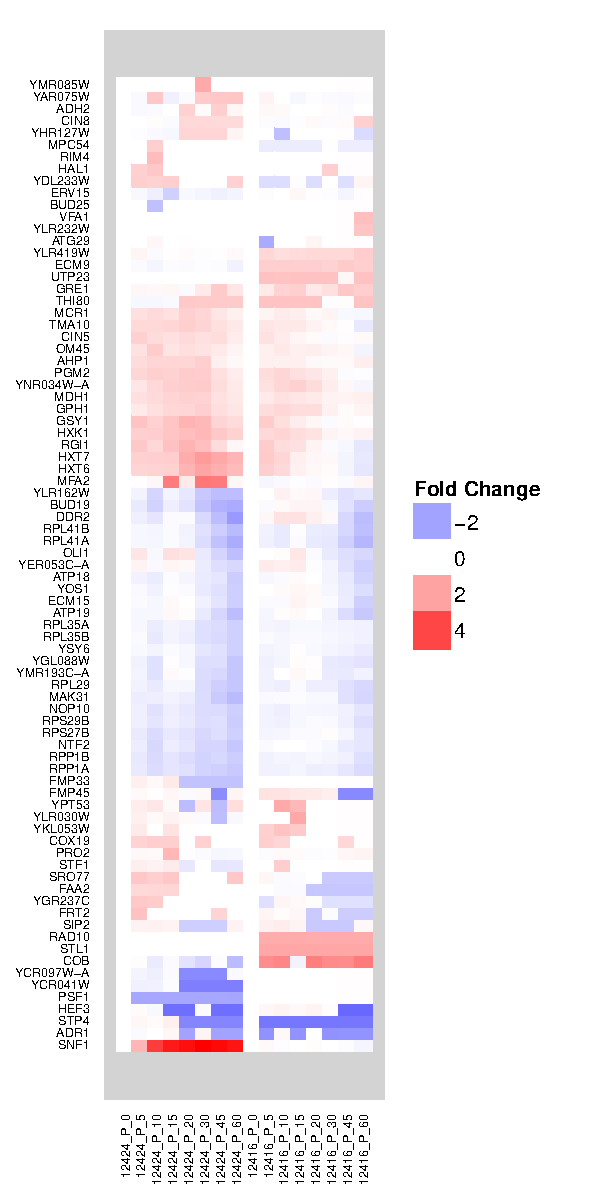
\includegraphics[width=\maxwidth]{figure/p1} 
\end{knitrout}

\caption{Phosphate-limited expression data. DBY12424 on left, DBY12416 (4ZEV control) on right.}
\end{figure}


\begin{figure}[hbtp]
\centering
\begin{knitrout}
\definecolor{shadecolor}{rgb}{0.969, 0.969, 0.969}\color{fgcolor}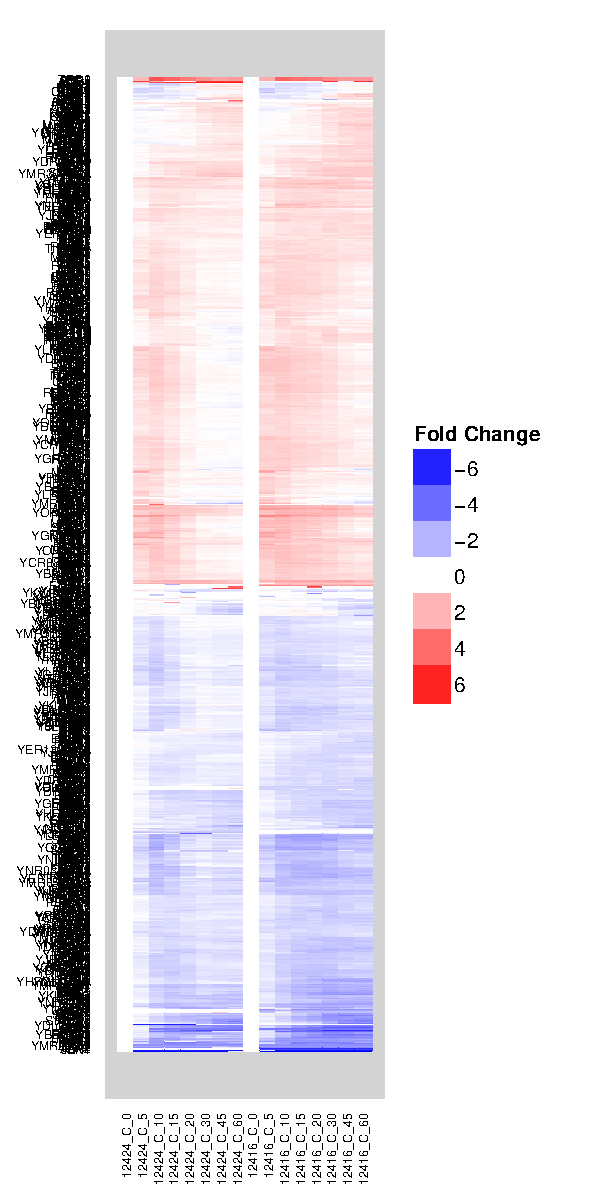
\includegraphics[width=\maxwidth]{figure/p2} 
\end{knitrout}

\caption{Carbon-limited expression data. 4ZEVpr-SNF1 on left, 4ZEV control on right.}
\end{figure}

There is significantly more signal in the 4ZEV control strain than expected, in both conditions. My first thought was that the samples were mislabeled, and I had accidentally labeled the experimental strain twice; however, looking at the expression data for \emph{SNF1}, you can see clearly that \emph{SNF1} expression changes only in the experimental strains and not in the control strains.
\begin{figure}[H]
\centering
\begin{knitrout}
\definecolor{shadecolor}{rgb}{0.969, 0.969, 0.969}\color{fgcolor}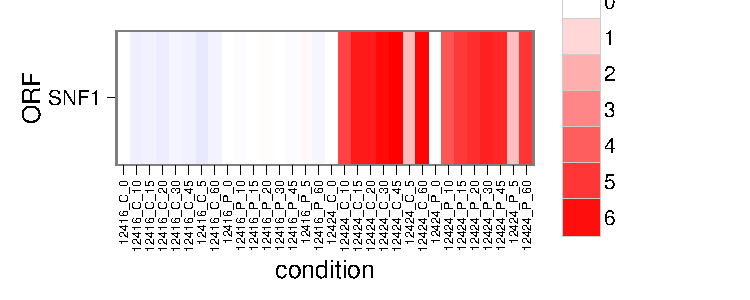
\includegraphics[width=\maxwidth]{figure/p3} 
\end{knitrout}

\end{figure}

%-------------------------------------------------------------------------------------------------------------------
\section*{Analysis of the 4-ZEV Arrays}
%-------------------------------------------------------------------------------------------------------------------

I'm not sure what to make of the control expression data. Obviously, some aspect of my experimental conditions is causing a significant gene expression response in both my control and experimental data. Because this response is more significant in my carbon-limited data (i.e., many more genes respond), I'm inclined to say that this expression change is due to some change in carbon-source availability. My preliminary guess is that the process of sampling (which I had tried to minimize by taking only 5 mL of culture for each timepoint rather than the standard 10 mL) is increasing the concentration of glucose available in the vessel, causing this gene expression response. This effect may be more significant at slower growth rates.

I decided to look at the zero timepoints for each chemostat, to see which genes were very highly differentially expressed across the conditions. The genes which make up the most significantly repressed cluster in the carbon-limited chemostats are \emph{PHO5}, \emph{PHM6}, \emph{SPL2}, \emph{PHO11}, \emph{PHO12}, and \emph{PHO84}. They are expressed at a much lower level than my reference RNA, a phosphate-limited chemostat at 0.15$hr^{-1}$. A cluster of genes which are highly-expressed in carbon-limited chemostats when compared to phosphate-limited chemostats includes \emph{HXT7}, \emph{HXT6}, \emph{ALD4}, and \emph{ADH2}, among other genes. There is not a significant difference in there expression in 4ZEVpr-SNF1 when compared to the 4ZEV control, indicating that these genes can be upregulated even in the absence of Snf1p. A quick GO-slim search on the cluster shows enrichment for transmembrane transport, carbohydrate metabolic process, generation of precursor metabolites and energy, and cofactor metabolic process.
\begin{figure}[hbtp]
\centering
\begin{knitrout}
\definecolor{shadecolor}{rgb}{0.969, 0.969, 0.969}\color{fgcolor}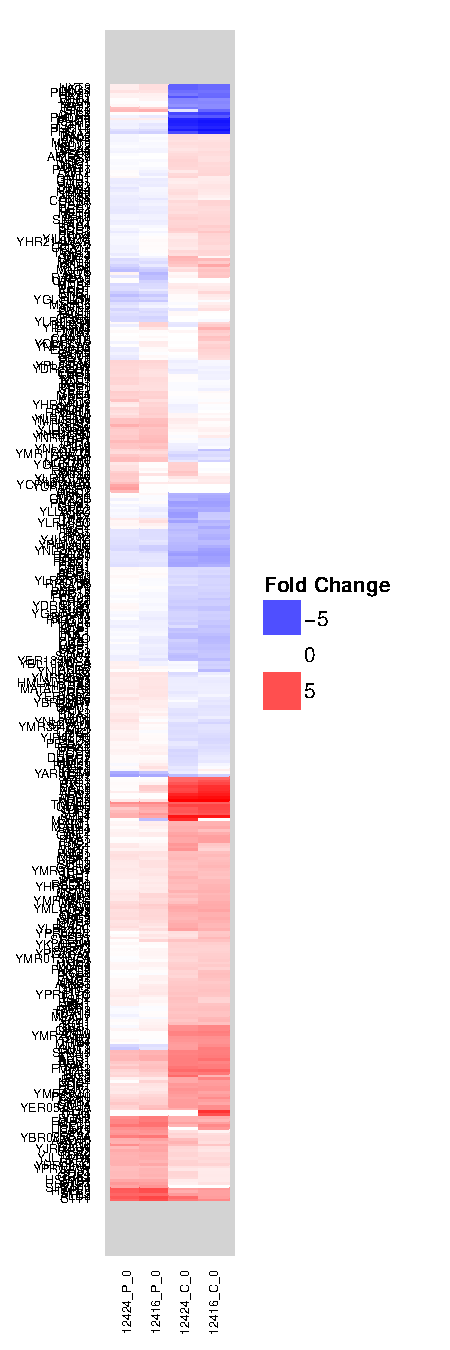
\includegraphics[width=\maxwidth]{figure/p4} 
\end{knitrout}

\caption{Expression of top 10\% of genes at time zero.}
\end{figure}

I decided to see what happened to this cluster of 35 genes that were already highly expressed at time zero in my carbon-limited samples. (Figure ~\ref{fig:carboncluster}) Over the course of the experiment, many of these genes are highly repressed in the carbon-limited vessels (with very similar expression patterns in both experimental and control), while there is not significant response in the phosphate-limited chemostats (with the exception of \emph{HXT7} and \emph{HXT6}). This repression of the cluster strongly resembles the typical response to a pulse of glucose, lending support to my idea that sampling the carbon-limited chemostats is increasing the available glucose, triggering a gene expression response.
\begin{figure}[here]
\centering
\begin{knitrout}
\definecolor{shadecolor}{rgb}{0.969, 0.969, 0.969}\color{fgcolor}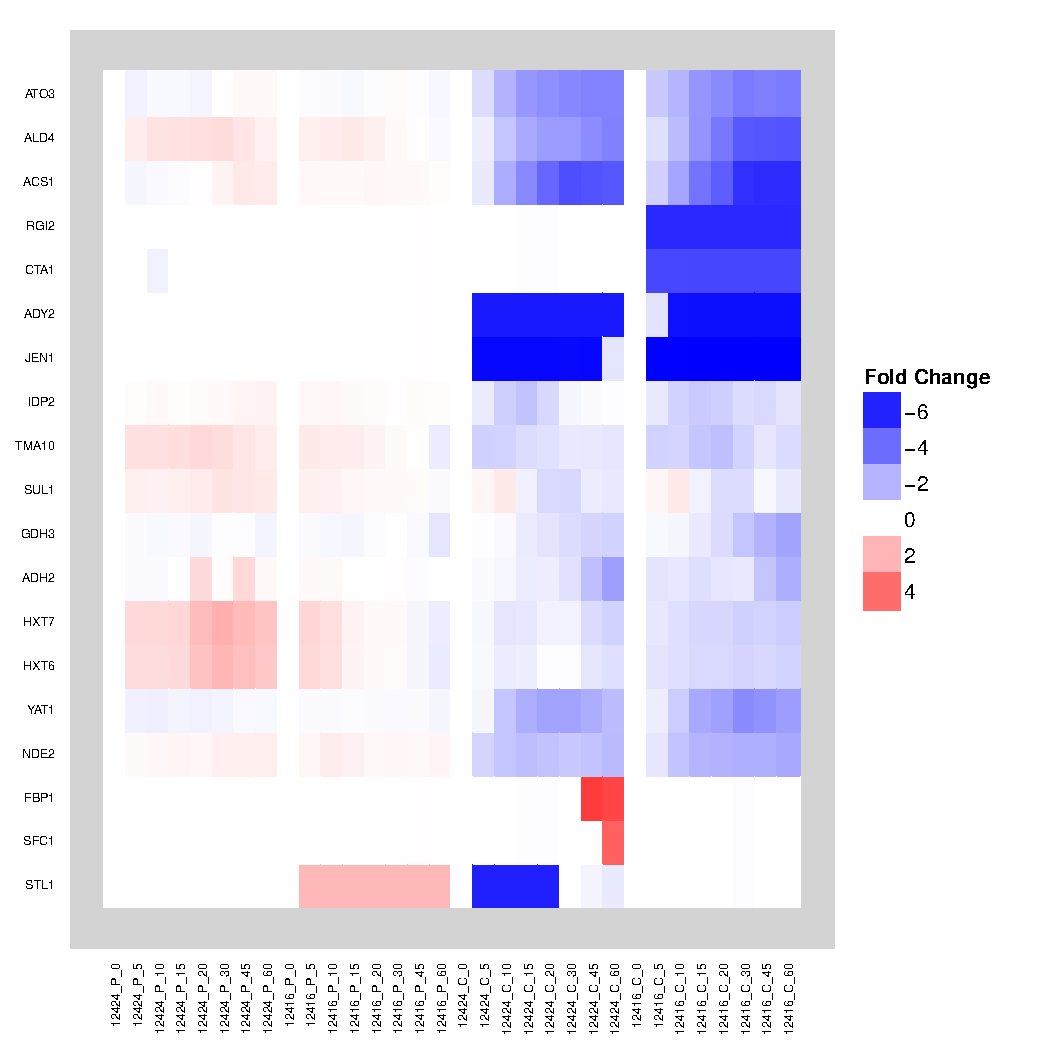
\includegraphics[width=\maxwidth]{figure/p5} 
\end{knitrout}

\caption{Expression time-course for genes which had basal high expression levels in the carbon-limited chemostats.}
\label{fig:carboncluster}
\end{figure}

\subsection*{SVD of 4-ZEV arrays}
I decided to see if subtracting the high control background would produce anything useful. There are three main eigengenes for both carbon and phosphate-limited control arrays, and they appear to be the reverse of each other (e.g., repression in carbon-limitation becomes activation in phosphate-limitation). It should also be noted that these three eigengenes account for a much smaller portion of the total expression fraction in the phosphate-limited chemostats, supporting the idea that the effect of sampling is much larger in carbon-limited chemostats than phosphate-limited chemostats. (Figures ~\ref{fig:csvd} and ~\ref{fig:psvd})
\begin{sidewaysfigure}
\centering
\begin{knitrout}
\definecolor{shadecolor}{rgb}{0.969, 0.969, 0.969}\color{fgcolor}\begin{kframe}
\begin{verbatim}
## Using eigengene as id variables
\end{verbatim}
\end{kframe}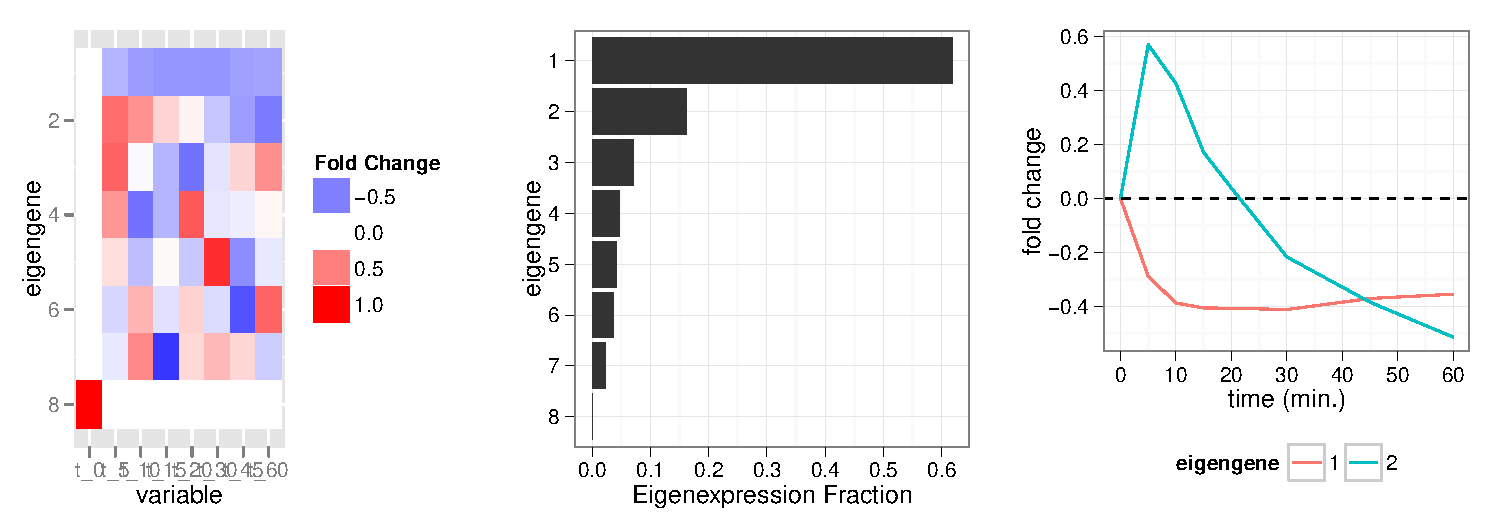
\includegraphics[width=\maxwidth]{figure/svd-carbon} 
\end{knitrout}

\caption{SVD on carbon-limited control arrays.}
\label{fig:csvd}
\end{sidewaysfigure}

\begin{sidewaysfigure}
\centering
\begin{knitrout}
\definecolor{shadecolor}{rgb}{0.969, 0.969, 0.969}\color{fgcolor}\begin{kframe}
\begin{verbatim}
## Using eigengene as id variables
\end{verbatim}
\end{kframe}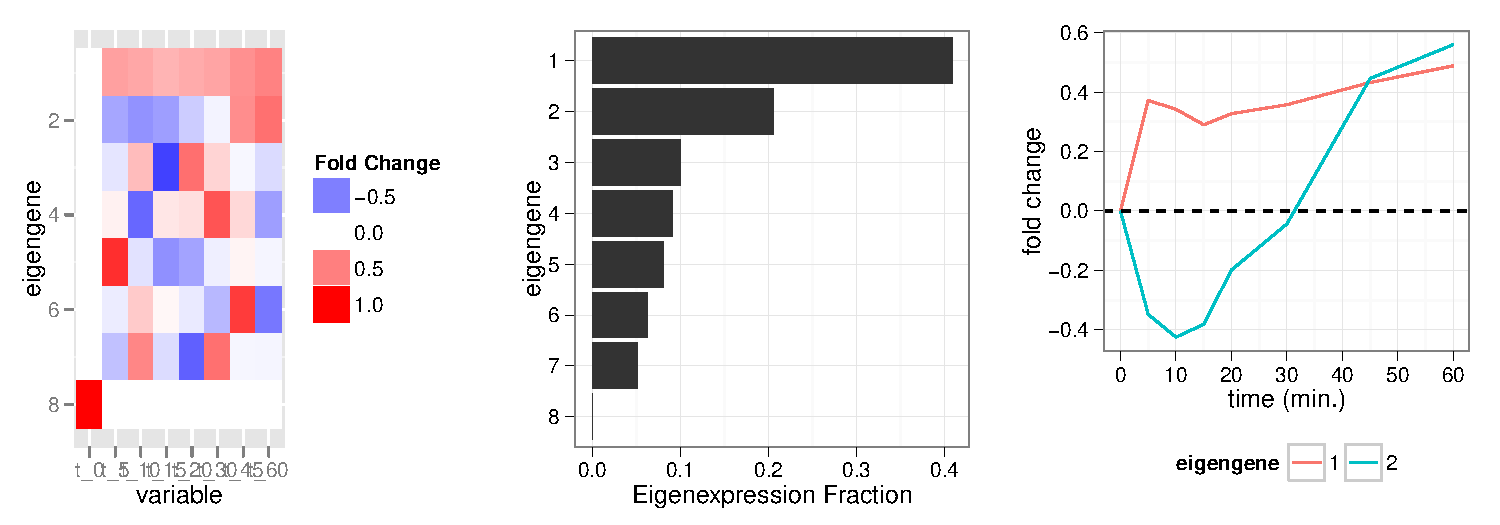
\includegraphics[width=\maxwidth]{figure/svd-phosphate} 
\end{knitrout}

\caption{SVD on phosphate-limited control arrays.}
\label{fig:psvd}
\end{sidewaysfigure}

\subsection*{Correlation of gene expression with eigengenes.}
I would like to know which genes in each of the 4ZEV arrays correspond to each of the top three eigengenes. To do so, I will correlate each gene's expression pattern with each of the top three eigengenes.

\begin{figure}
\begin{knitrout}
\definecolor{shadecolor}{rgb}{0.969, 0.969, 0.969}\color{fgcolor}\begin{kframe}
\begin{verbatim}
## [1] 10
## [1] 10
\end{verbatim}
\end{kframe}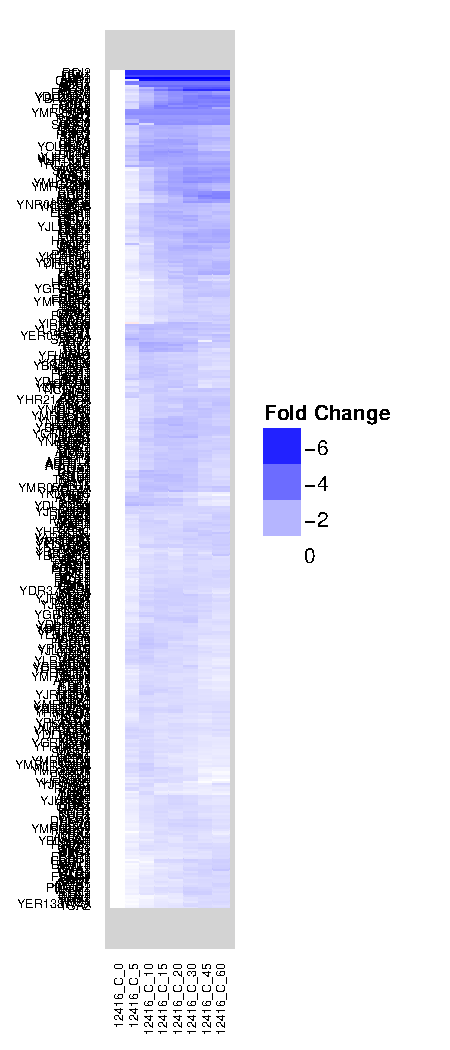
\includegraphics[width=\maxwidth]{figure/eigengenes-carbon1} 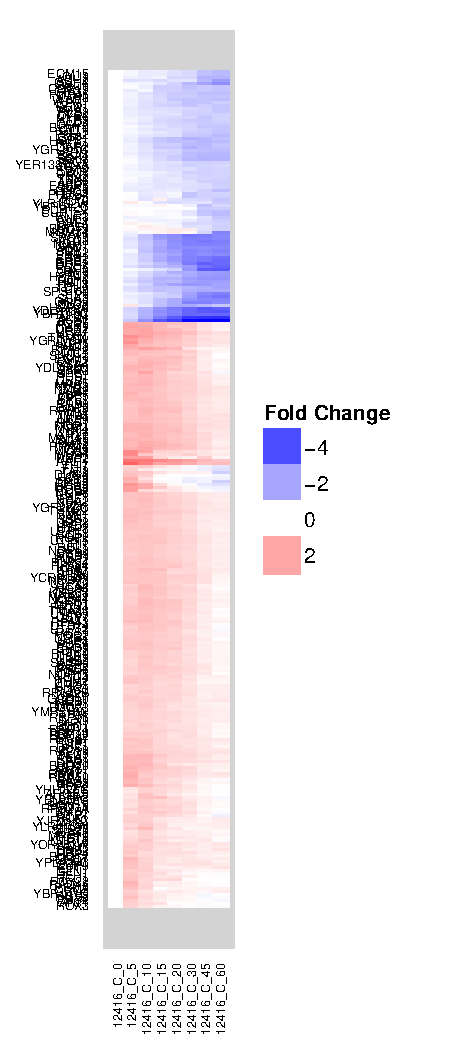
\includegraphics[width=\maxwidth]{figure/eigengenes-carbon2} 
\end{knitrout}

\caption{Expression patterns of genes correlated with eigenvector 1 (left) and eigenvector 2 (right) for carbon-limited 4ZEV strains.}
\end{figure}


\begin{figure}
\begin{knitrout}
\definecolor{shadecolor}{rgb}{0.969, 0.969, 0.969}\color{fgcolor}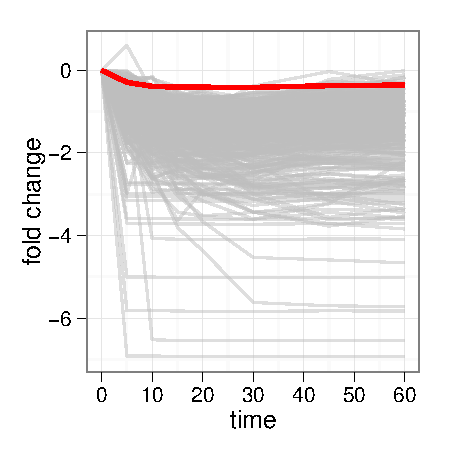
\includegraphics[width=\maxwidth]{figure/ploteigs1} 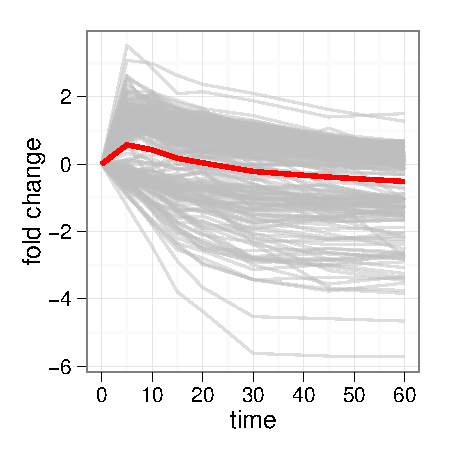
\includegraphics[width=\maxwidth]{figure/ploteigs2} 
\end{knitrout}

\caption{Expression patterns of genes correlated with eigenvector 1 (left) and eigenvector 2 (right) for carbon-limited 4ZEV strains.}
\end{figure}

There appear to be two eigengenes that explain the majority of the variance in the carbon-limited 4ZEV chemostat time course. The main is a strong repression signal, and the second appears to be brief induction followed by lasting repression. When I identified genes whose signal was correlated with each eigengene (using a p-value of 0.05 calculated by permutation testing), eigenvector 2 appears to be actually made up of two different clusters: one cluster consistening of genes who appear to be undergoing a delayed repression, and one of a rapid and transient induction.

I used SGD's GOSlim tool to test for GO term enrichment in each group, and found that many of the genes in clustering with eigengene 1 are of biological process unknown, carbohydrate metabolic process(AMS1, ARA1, ATH1, CDC19, CIT2, ENO1, ENO2, FBA1, GCY1, GDB1, GID7, GLC3, GLG1, GLK1, GND1, GND2, GPH1, GPM1, GRE3, GSY1, GSY2, GUT1, GUT2, HSP104, HXK1, IGD1, IMA1, MDH3, NDE2, NTH2, OPI10, PDC1, PFK1, PFK26, PGI1, PGK1, PGM2, PIG2, PSK1, SHC1, SOL3, SOL4, TAL1, TDH1, TDH2, TDH3, TKL2, TPI1, TPS1, TPS2, TPS3, TSL1, UBC8, UGP1, VID28, VID30, YJR096W, YLR345W, YPR1
), response to chemical stimulus (ACT1, ADR1, AHP1, BXI1, CCP1, CCW12, CDC48, CTA1, CTT1, ETP1, GAD1, GCY1, GND1, GRE3, GRX2, HBT1, HSP104, HSP12, HYR1, KIN82, LAP3, MCR1, MDG1, PDR10, PDR15, PRX1, ROD1, SNQ2, SOD1, SPI1, TRR2, TRX2, TRX3, TSA2, UGA2, USV1, YDL124W, YJR096W, YPR1), and generation of precursor metabolites and energy (AAC1, ACS1, CDC19, CIT1, ENO1, ENO2, ETR1, FBA1, GDB1, GLC3, GLG1, GLK1, GPH1, GPM1, GSY1, GSY2, HXK1, IGD1, ISF1, LSC1, NDE2, PDC1, PET10, PFK1, PFK26, PGI1, PGK1, PGM2, PIG2, PSK1, RGI1, RGI2, SHY1, TDH1, TDH2, TDH3, TPI1, UGP1, YLR345W).

For eigengene 2, the cluster which is repressed is enriched in cellular amino acid metabolic process (ADH2, ALD2, ALD3, CAR2, GAD1, GDH3, GLT1, GTT1, LAP3, PDC6, YAT1), nucleobase containing small molecule metabolic process (ADH2, ALD4, ATP6, GND2, IRA2, OLI1, RNR3, SOL3, TKL2), response to chemical stimulus (GAD1, HBT1, HSP12, HYR1, LAP3, SPI1, TRX3, TSA2), and carbohydrate metabolic process (CDC19, GND2, SHC1, SOL3, TDH2, TDH3, TKL2).

The cluster which is transiently activated is highly enriched in rRNA processing, various terms associated with ribosomal biogenesis.

I am also interested in seeing how my data correspond to the 2006 Ronen paper, so I will subset the data associated with each gene expression pattern she observed.

\begin{figure}
\centering
\begin{knitrout}
\definecolor{shadecolor}{rgb}{0.969, 0.969, 0.969}\color{fgcolor}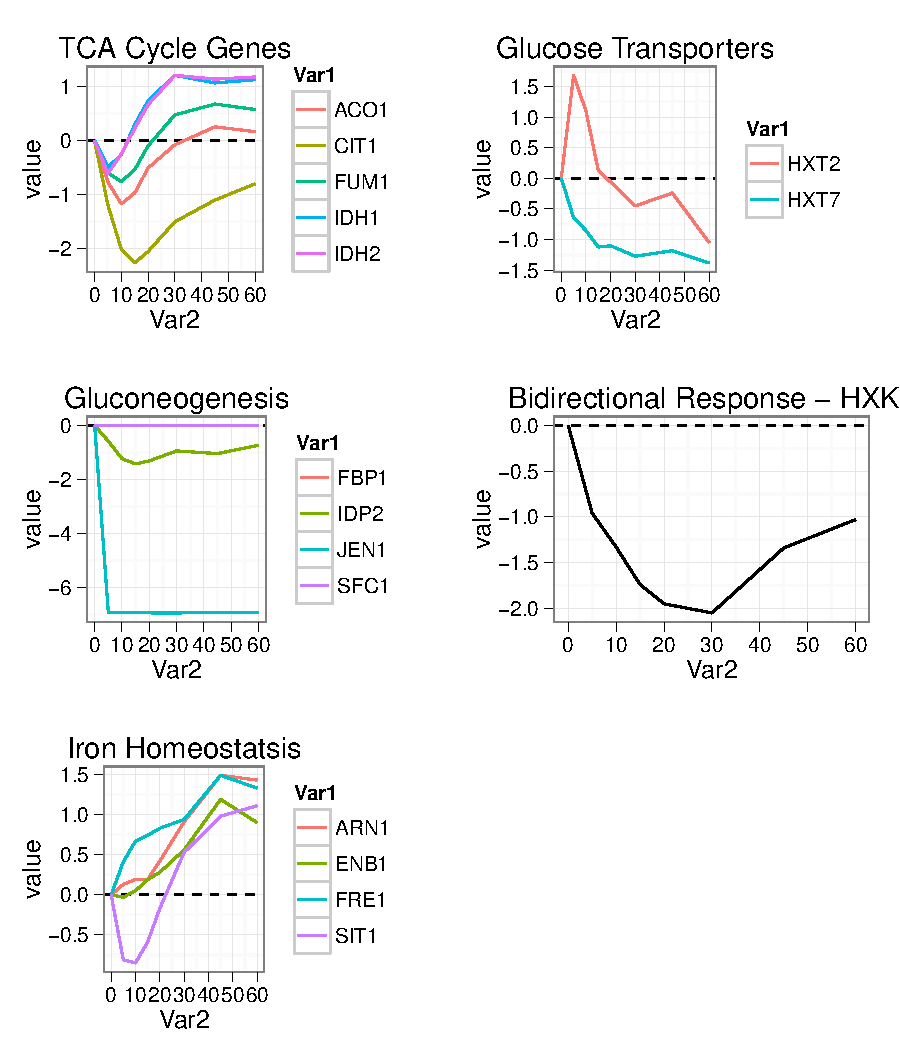
\includegraphics[width=\maxwidth]{figure/ronengenes} \begin{kframe}\begin{verbatim}
## NULL
\end{verbatim}
\end{kframe}
\end{knitrout}

\caption{Expression of genes in the Carbon-limited 12416 chemostats from clusters identified in Ronen 2006.}
\end{figure}

\begin{figure}
\begin{knitrout}
\definecolor{shadecolor}{rgb}{0.969, 0.969, 0.969}\color{fgcolor}\begin{kframe}
\begin{verbatim}
## [1] 10
## [1] 10
## [1] 10
\end{verbatim}
\end{kframe}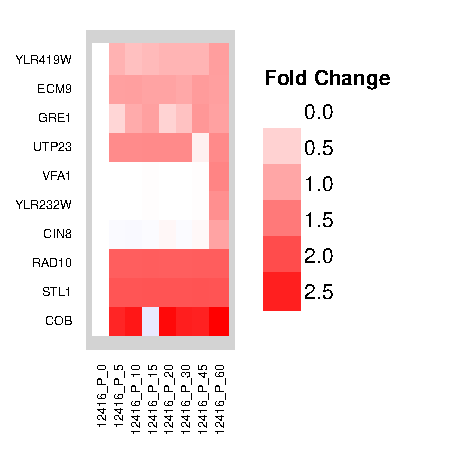
\includegraphics[width=\maxwidth]{figure/eigengenes-phosphate1} 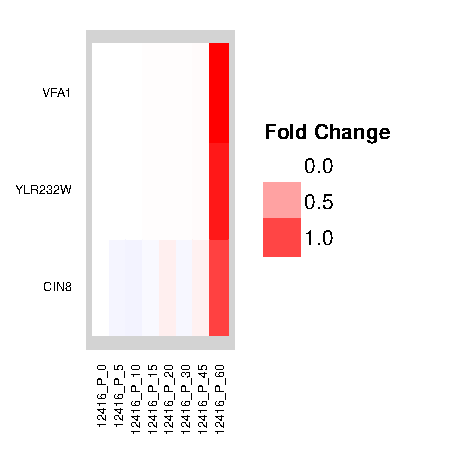
\includegraphics[width=\maxwidth]{figure/eigengenes-phosphate2} 
\end{knitrout}

\caption{Expression patterns of genes correlated with eigenvector 1 (left) and eigenvector 2 (right) for phosphate-limited 4ZEV strains.}
\end{figure}

\begin{figure}
\begin{knitrout}
\definecolor{shadecolor}{rgb}{0.969, 0.969, 0.969}\color{fgcolor}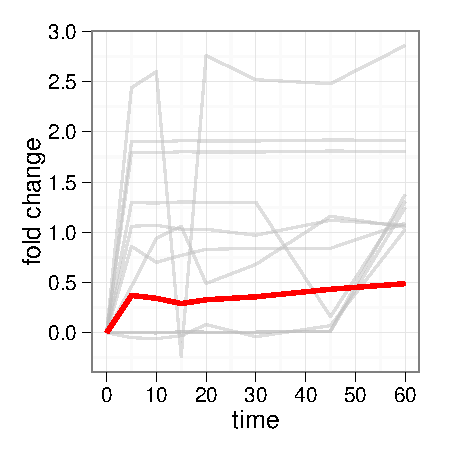
\includegraphics[width=\maxwidth]{figure/w1} 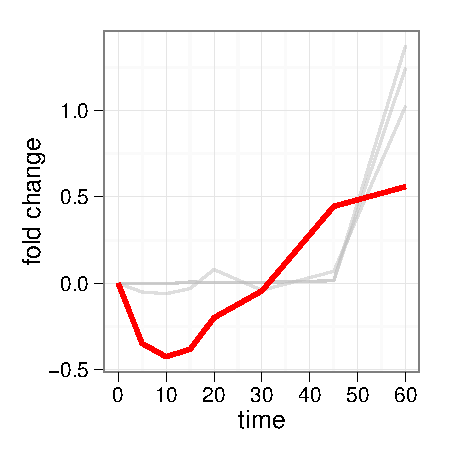
\includegraphics[width=\maxwidth]{figure/w2} 
\end{knitrout}

\caption{Expression patterns of genes correlated with eigenvector 1 (left) and eigenvector 2 (right) for phosphate-limited 4ZEV strains.}
\end{figure}

%-------------------------------------------------------------------------------------------------------------------
\section*{Analysis of 4ZEV$_{pr}$-SNF1 data with 4ZEV signal removed.}
%-------------------------------------------------------------------------------------------------------------------
\begin{figure}
\centering
\begin{knitrout}
\definecolor{shadecolor}{rgb}{0.969, 0.969, 0.969}\color{fgcolor}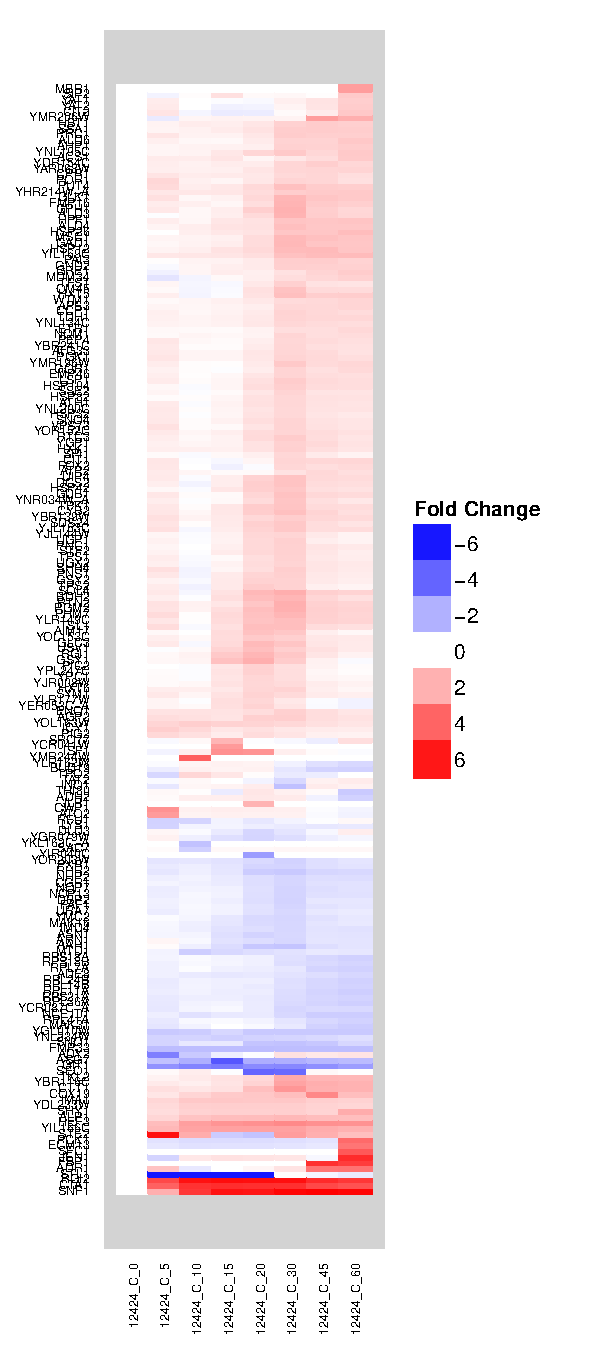
\includegraphics[width=\maxwidth]{figure/p8} 
\end{knitrout}

\caption{Carbon-limited 4ZEVpr-SNF1 with control top two eigengenes subtracted}
\end{figure}

\begin{figure}
\centering
\begin{knitrout}
\definecolor{shadecolor}{rgb}{0.969, 0.969, 0.969}\color{fgcolor}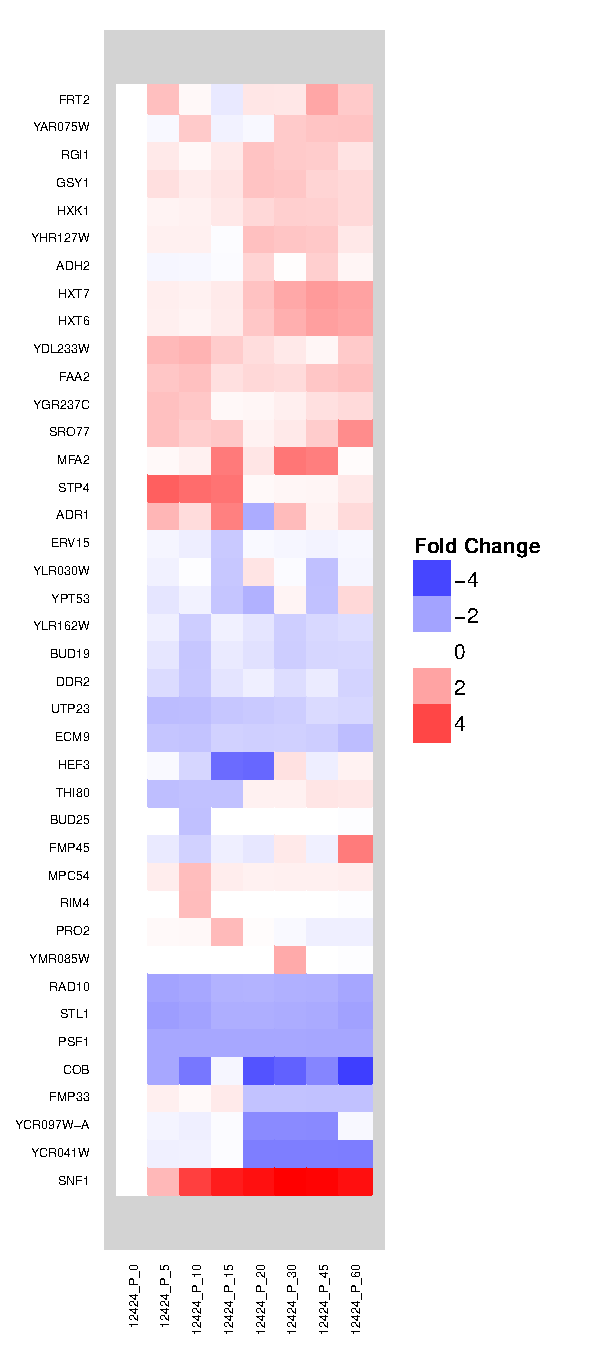
\includegraphics[width=\maxwidth]{figure/p9} 
\end{knitrout}

\caption{Phosphate-limited 4ZEVpr-Snf1 with control top two eigengenes subtracted}
\end{figure}

After subtracting the top-three eigengenes of the respective control data sets from the experimental data sets, there are still 194 genes which change by at least 2-fold in the carbon-limited data set, and 40 genes which change by at least 2-fold in the phosphate-limited data set. There are 16 genes which change by at least 2-fold in both conditions.
\begin{kframe}
\begin{flushleft}
\ttfamily\noindent
\hlsymbol{tab}{\ }\hlassignement{=}{\ }\hlfunctioncall{xtable}\hlkeyword{(}\hlfunctioncall{data.frame}\hlkeyword{(}\hlargument{ORF}{\ }\hlargument{=}{\ }\hlfunctioncall{unlist}\hlkeyword{(}\hlfunctioncall{orf2name}\hlkeyword{(}\hlfunctioncall{intersect}\hlkeyword{(}\hlfunctioncall{rownames}\hlkeyword{(}\hlsymbol{p.424.new}\hlkeyword{)}\hlkeyword{,}\hspace*{\fill}\\
\hlstd{}{\ }{\ }{\ }{\ }\hlfunctioncall{rownames}\hlkeyword{(}\hlsymbol{c.424.new}\hlkeyword{)}\hlkeyword{)}\hlkeyword{)}\hlkeyword{)}\hlkeyword{)}\hlkeyword{)}\hspace*{\fill}\\
\hlstd{}\hlfunctioncall{print}\hlkeyword{(}\hlsymbol{tab}\hlkeyword{,}{\ }\hlargument{tabular.environment}{\ }\hlargument{=}{\ }\hlstring{"{}longtable"{}}\hlkeyword{,}{\ }\hlargument{floating}{\ }\hlargument{=}{\ }\hlnumber{FALSE}\hlkeyword{,}{\ }\hlargument{include.rownames}{\ }\hlargument{=}{\ }\hlnumber{FALSE}\hlkeyword{)}\mbox{}
\normalfont
\end{flushleft}
\end{kframe}
% latex table generated in R 2.15.1 by xtable 1.7-0 package
% Mon Aug 27 13:32:44 2012
\begin{longtable}{l}
  \hline
ORF \\ 
  \hline
HXK1 \\ 
  YCR041W \\ 
  ADH2 \\ 
  HXT6 \\ 
  STL1 \\ 
  SRO77 \\ 
  FMP33 \\ 
  BUD19 \\ 
  ADR1 \\ 
  GSY1 \\ 
  YDL233W \\ 
  RGI1 \\ 
  THI80 \\ 
  SNF1 \\ 
  HEF3 \\ 
  YLR162W \\ 
   \hline
\hline
\end{longtable}





\end{document}
